%%%%%%%%%%%%%%%%%%%%%%% file template.tex %%%%%%%%%%%%%%%%%%%%%%%%%
%
% This is a general template file for the LaTeX package SVJour3
% for Springer journals.          Springer Heidelberg 2010/09/16
%
% Copy it to a new file with a new name and use it as the basis
% for your article. Delete % signs as needed.
%
% This template includes a few options for different layouts and
% content for various journals. Please consult a previous issue of
% your journal as needed.
%
%%%%%%%%%%%%%%%%%%%%%%%%%%%%%%%%%%%%%%%%%%%%%%%%%%%%%%%%%%%%%%%%%%%
%
% First comes an example EPS file -- just ignore it and
% proceed on the \documentclass line
% your LaTeX will extract the file if required
\begin{filecontents*}{example.eps}
%!PS-Adobe-3.0 EPSF-3.0
%%BoundingBox: 19 19 221 221
%%CreationDate: Mon Sep 29 1997
%%Creator: programmed by hand (JK)
%%EndComments
gsave
newpath
  20 20 moveto
  20 220 lineto
  220 220 lineto
  220 20 lineto
closepath
2 setlinewidth
gsave
  .4 setgray fill
grestore
stroke
grestore
\end{filecontents*}
%
\RequirePackage{fix-cm}
%
%\documentclass{svjour3}                     % onecolumn (standard format)
%\documentclass[smallcondensed]{svjour3}     % onecolumn (ditto)
% \documentclass[smallextended]{svjour3}       % onecolumn (second format)
\documentclass[twocolumn]{svjour3}          % twocolumn
%
\smartqed  % flush right qed marks, e.g. at end of proof
%
\usepackage{graphicx}
%
% \usepackage{mathptmx}      % use Times fonts if available on your TeX system
%
% insert here the call for the packages your document requires
%\usepackage{latexsym}
% etc.
%
% please place your own definitions here and don't use \def but
% \newcommand{}{}
%
% Insert the name of "your journal" with
% \journalname{myjournal}
%

\usepackage[abbreviations]{foreign}
\usepackage{bbm}
\usepackage{amsmath}
% \usepackage{cleveref}
\usepackage{glossaries-extra}
\PassOptionsToPackage{language=auto,backref=true,urldate=iso,seconds=true,date=iso, datamodel=custom,datecirca=true, dateuncertain=true}{biblatex}
   \usepackage{biblatex}
   \addbibresource{mybibfile.bib}
   \usepackage{paralist}
   \usepackage{tabularx}
   \usepackage{csquotes}
   \usepackage{booktabs}
   \usepackage{hyperref}
   \usepackage[utf8]{inputenc}
   \usepackage[hyperref,framed]{ntheorem}
   \newtheorem{hypo}{Hypothesis}
   \PassOptionsToPackage{pdftex,hyperfootnotes=false,pdfpagelabels,bookmarksdepth=3}{hyperref}
%    \crefname{hypo}{Hypothesis}{Hypotheses}
   \usepackage[all]{hypcap}
   \usepackage{hyphenat}
   \hypersetup{ colorlinks=false, linktocpage=true}

\begin{document}

\title{The Benefits of Adaptive Robots Compared to Adaptable Robots%\thanks{Grants or other notes
%about the article that should go on the front page should be
%placed here. General acknowledgments should be placed at the end of the article.}
}
\subtitle{Using Dueling Bandit Learning to Learn Users' Task Preferences in HRI}

%\titlerunning{Short form of title}        % if too long for running head

\author{Sebastian Schneider         \and
        Franz Kummert %etc.
}

%\authorrunning{Short form of author list} % if too long for running head

\institute{F. Author \at
              first address \\
              Tel.: +123-45-678910\\
              Fax: +123-45-678910\\
              \email{fauthor@example.com}           %  \\
%             \emph{Present address:} of F. Author  %  if needed
           \and
           S. Author \at
              second address
}

\date{Received: date / Accepted: date}
% The correct dates will be entered by the editor


\maketitle

\begin{abstract}
  Learning and matching a user's preference is an essential aspect of achieving a productive collaboration in long-term Human-Robot Interaction. However, there are different techniques on how to match the behavior of a robot to a user's preference. The robot can be adaptable so that a user can change the robot's behavior to ones need, or the robot can be adaptive and autonomously tries to match its behavior towards a user's preference. Both types might lead to the same preference matching results. However, the Level of Automation (LoA) of the robot is different between both methods. Either the user controls the interaction, or the robot is in control. In this paper, we present a study on the effects of these different LoA of a Socially Assistive Robot (SAR) on a user's evaluation of the system in an exercising scenario. We conducted a between-subject design study (adaptable robot vs. adaptive robot) with 40 subjects. The results show that users evaluate the adaptive robots as more competent, warm and report a higher alliance. Moreover, this increased alliance is significantly mediated by the perceived competence of the system. This result provides empirical evidence for the relation between the LoA of a system, the user's perceived competence of the system and the perceived alliance with it.
\end{abstract}

\section{Introduction}
\label{intro}
Future scenarios of socials robots envision a personalizable system that is flexible and adapts itself to the user's preferences[@@leite].
% <!-- without the need to program the desired behavior.  -->
% <!-- and at best knows what the user wants without the need to program the desired behavior.  -->
% <!-- Having adaptive robots is an essential requirement for long-term interaction with social robots [@leite].  -->
Since it is not possible to anticipate every potential user and pre-program the system for their needs, robots will potentially need to have capabilities to adjust to different users (\eg{}, match a user's personality \cite{andrist2015look}). 
% <!-- For example, robots might enhance the interaction experience by adjusting behaviors that match the personality of the user [@andrist2015look]. -->
Adapting to different users and enhancing the interaction is already successfully implemented in web-based applications (e.g., recommender systems on Amazon, Google, eBay). However, adaptation remains a challenging issue for social robots that is not attached to a user database which could enable techniques like collaborative filtering. 
Therefore, social robots will face a cold start problem, which requires the system to gather initial user data. 
Hence, deploying an adaptive system comes with some difficulties: 

First, querying the user for information in real time HRI might be more cost-intensive than in web-based applications. 
Cakmak et al. \cite{cakmak2010designing} showed that a constant stream of questions in a Learning by Demonstration (LbD) task annoys users. 

Second, when the robot starts to make autonomous personalization decisions, it might cause concerns for the HRI experience, 
Accordingly, it could be sufficient for the human to adjust the required behavior instead of having the robot adapt by itself. 
This different types of possible personalization strategies would influence the autonomy of the system, which in turn might affect the interaction experience in different ways.
%  <!-- \footnote{I mean autonomy in the sense that the system either controls itself or is controlled by the user. We also associate autonomy with the system's capabilities to adapt autonomously or to be adaptable by the user}  -->

Based on the theory of anthropomorphization, an autonomous adaptive system could create an unexpected experience for the user [@epley2007seeing]. This unexpected experience could increase a user's perceived anthropomorphization of the robot. Furthermore, this higher degree could enhance the credibility of the system and might influence the trust in it. 
In contrast, a system that is controlled and adjusted by the user should increase the match between the robot's behavior and the user's expectation and therefore reduce anthropomorphic effects. 
The investigation of these two aspects is the core of this work. We try to find an answer to the question: 

What effects have different types of preference learning robots on the user's acceptance, relationship and motivation to interact with the system?

To investigate the effects of different preference matching behaviors of the system this work presents a study that compares the impact of having an adaptive robot or an adaptable robot as an exercising partner for physical activities. Previous work on robots for exercising and coaching have investigated the motivational effects of using such coaching systems \cite{fasola2013socially,schneider2016exercising,guneysu2017}. However, most of the previous studies used only one type of exercises (\eg{}, arm or plank exercises). Thus, the users could not choose between different exercises. In this work, we present a system that offers a range of exercises to the users and raise the question of what is a suitable preference matching framework to provide a personalized interaction for the user. Therefore, in the adaptive condition, the robot proposes different activities for the user and tries to learn an exercising category preference of the user based on preference feedback. In the adaptable condition, the robot is directly controlled by the user, and the user can always decide what kind of exercises they want to do together with the robot.

The difference between adaptive and adaptable robots will be explained in \autoref{adaptation:sec:background} along with the concepts of automation and relationship, which might be important variables when looking at the adaptivity of a system. \autoref{adaptation:sec:system} introduces the system design and \autoref{adaptation:sec:study} explains the study design to test the effects of a robot's different personalization mechanisms. \autoref{adaptation:sec:results} presents the results of the study, which are discussed in \autoref{adaptation:sec:discussion}. Finally, \autoref{adaptation:sec:conclusion} gives a conclusion of this work.

\section{Adaptation, Automation and Alliance} \label{adaptation:sec:background}
This section gives a brief introduction into the concepts of adaptation, automation and alliance. Discussing these topics is a challenging task because they are used differently across disciplines (\eg{}, philosophy, psychology, economics, biology). Therefore, the following explanations can not be exhaustive and will focus mainly on a computer science and psychology perspective.
 

% <!-- that were not introduced yet, but might be important for the interaction with social robots in the future.  -->
% <!-- Grasping these concepts is challenging because they have different meanings and definitions in different disciplines (\eg{}, philosophy, psychology, economics, biology). -->
% <!-- However, contrasting them and defining will be helpful to understand this work and the impact of the results. -->
% <!-- Nevertheless, the sketching of these concepts cannot be exhaustive due to the broad range of disciplines using these terms. Therefore, we will concentrate and look on the terms from a computer science and psychology perspective. -->

\subsection{Adaptation: adaptivity versus adaptability}
In computer science adaptation is the process of adjusting the behavior of an interactive system to individuals using information about them. 
Even though computer software or robots are running through many software design cycles, it is hard to anticipate the requirements for every possible user. 
The goal of the adaptive process is to minimize the discrepancy between the user needs and system behavior after the deployment.
This adaptive process can either be automatically initiated by the system, in this case, the system is adaptive (\eg{}, the system chooses exercises for the users by itself), or users can adjust the system by themselves, in this case the system is adaptable (\eg{}, the users can choose the exercises by themselves). 
Adaptation can be based on different user profiles (\eg{}, age, gender, personality), various times (\eg{}, morning/evening, days of the week, summer/winter) or other user characteristics (\eg{}, mood, expertise over time). 

% <!-- Previous work in the area of adaptation and personalization  -->

% <!-- The previous chapter already introduced some of the related work in the area of adaptation and personalization in HRI. Therefore, these works are not listed here again. However, there is a lack of knowledge in the research community because few works compared different possibilities to match a robot's behavior to the user needs. -->

Previous work in HRI investigated the implementation of adaptive processes to match a user's personality, generate empathic behavior, adapt therapy sessions, interaction distance, or puzzle skills.  \cite{tapus2008user,leite2011modelling,Tsiakas2016,mitsunaga2008adapting,leyzberg2014personalizing}. Although some have compared adaptive robots with experimental baseline control conditions (\eg{}, [@leyzberg2014personalizing]), to the best of our knowledge, no works looked at the effects of robot-initiated personalization versus user-initiated personalization. 
It is reasonable to argue that the users could control and adjust the robot behavior to their preferences. Leyzberg et al. [@leyzberg2014personalizing], for example, investigated the effects of a robot that gives personalized lessons to the user. These tutorials are selected by the robot's decisions. However, also the user could have requested for a specific lesson.  

Both strategies might might match a user's preference and increase the interaction satisfaction, but the underlying difference in decision making is fundamental. One can interpret the different strategies as either more transparent or as more competent. 
Generally, the question of whether to build an adaptive or adaptable system raises the concern of who is in control and how does it affect the interaction experience. The issue of who is in control is associated with the Level of Automation (LoA) of the system.

\subsection{Level of Automation}
An autonomous agent acts based on the information it receives from its sensors, knows in which state it is and makes a decision accordingly which is associated with an agent's action \cite{russell2016artificial}.
LoA of a system changes an agent's capability to act and react based on information on its own without any other external control instances.
Thus, the LoA of an agent is altered by the task and environment of the agent and whether a human can interfere with an agent's control loop. 

It becomes essential were robots are carrying out delicate tasks (\eg{}, lethal autonomous weapons). There are various frameworks that can be used to identifiy the LoA of a system (\eg{},\cite{sheridan1978human,endsley1995out}). However, most recently, \cite{beer2014toward} have proposed a taxonomy to classify the level of robot autonomy for HRI. 

Regardless of the exact different LoA, systems can be categorized as human-in-the-loop systems where the human has to approve a control decision by the autonomous agents, human-on-the-loop where the human is informed about decision but the agent would carry out a decision if the human operator is not interfering or  human-off-the-loop, where a human cannot interfere with the agent's decisions\footnote{Earliest examples of hands-off-the-loop agents are land and naval mines.}.


  The relevance to consider different LoA are apparent in sensible domains such as military operations or medical applications (\eg{}, surgery or medicine dispenser), but (yet) less apparent in socially assistive domains (\eg{}, rehabilitation or teaching).
Nevertheless, also social situations will require to understand whether a social robot should act autonomously, semi-self controlled or is in full human control. For the interaction experience it will be crucial to understand the effects of different LoA.
In the course of this work, we are interested in the effects of whether a robot exercising companion is in control to choose the exercises or the users can decide which exercises they want to do. 
The question of whether the LoA is appropriate and which effects it will have on the interaction will be related to the relationship and trust between the users and the Socially Assistive Robot (SAR) [@beer2014toward].


\subsection{Alliance and Trust}
Trust in HRI has recently been investigated in use cases in which a robot shows a faulty behavior, gives explanations for actions, or varies the degree of expressivity and vulnerability \cite{salem2015would,robinette2016overtrust,Wang,Martelaro}
% <!-- The influence of a robot's behavior on alliance and trust in HRI have previously been investigated from a point of view where the robot is showing a faulty behavior [@salem2015would;@robinette2016overtrust]. -->
Besides these aspects, it is also a significant issue of whether humans trust a robot's capabilities if it makes autonomous decisions \cite{freedy2007measurement}.
% <!-- In cases where systems have more control and decide on their own, either directly or controlled by the feedback of users, the relationship between the human and robot might influence the trust users put in the system's decision.  -->
% <!-- @dictionary2018merriam defines trust as 'the assured reliance on the character, ability, strength or truth of someone or something' [@dictionary2018merriam].  -->

Trust is defined Human-Computer Interaction (HCI) as 'the extent to which a user is confident in and willing to act by, the recommendations, actions, and decisions of an artificially intelligent decision aid' \textcite{mcallister1995affect} p. 25. As \textcite{madsen2000measuring} state, this definition  'encompasses both the user's confidence in the system and their willingness to act on the system's decision and advice' \cite[1]{madsen2000measuring}. Thus, it already incorporates a notion of user trust regarding the willingness to take a system's recommendations into account.

To understand how trust influences HRI, \textcite{hancock2011meta} reviewed different applications where confidence is an essential factor when robots and humans are working together in a team. They state that it is a crucial aspect of industry, space or warfare applications. Additionally, trust will also be essential to understanding social tasks due to the rise of SAR for rehabilitative, therapeutic or educational tasks \cite{corry,fasola2013socially}. Hancock et al. found several factors influencing trust in HRI, which are related to the human, the robot, and the environment. However, the robot related factors were the most important ones in their meta-review. They found that essential factors influencing the associated trust are the human's perception of the system's behavior, adaptability, competence, and performance \cite{hancock2011meta}.
Considering how different types of personalization change the LoA and how this might alter the perceived trust, we question how the manipulation of the LoA (for example how the system adapts or can be adapted) influences the associated competence and the perceived confidence in the system.

\textcite{rau2013effects} investigated the influence of a social robot's LoA on the user's trust in a robot and the influence on decision making. They manipulated the robot's LoA by either giving the human the possibility to make a team decision and the robot could suggest a different decision (low autonomy) or the robot makes the team decision and the human can either reject or accept this decision (high autonomy). They hypothesized that a highly autonomous robot would increase the associated trust. Their results show the influence of an autonomous robot on human's decision making, but in contrast to the hypothesis, people rated that they trust the low autonomous robot more. 

Other works investigated how perceived anthropomorphization influenced perceived trust in autonomous vehicles \textcite{waytz2014mind}. \textcite{waytz2014mind} found that the degree of anthropomorphization is associated with higher confidence in its competence. This indicates that the perceived level of skill might also influence the related trust. However, there is, to the best of our knowledge no other works that investigated the influence of a social robot's LoA on the perceived trust and competence besides the work of \textcite{rau2013effects}.

\subsection{Hypotheses}
Based on the reviewed literature, this work investigates the effects of preference adaptation with different LoA in HRI. We propose the following hypotheses:

\begin{hypo}\label{hyp:adaptability:competence}
 Users perceive an adaptive robot as more competent than an adaptable robot.
\end{hypo}

Due to the robot's initiative and control of the interaction people will be likely to associate the robot with higher competence. Since users do not have to control the robot on their own, the robot creates the impression of proactively deciding on its own. We hypothesize that this different level of perceived competence is associated with the perceived trust or relationship with the agent.

\begin{hypo}\label{hyp:adaptability:trust}
 The relationship to an adaptive robot is rated better than to an adaptable robot.
\end{hypo}

We base this hypothesis on the assumption that the users will more likely trust a system that is perceived by the users as competent. Even though research from \textcite{rau2013effects} did not show any significant effects on perceived trust depending on the LoA, we still hypothesize that the Level of Automation will affect the associated trust. 
It is likely that \textcite{rau2013effects} did not find an effect on the trust because the robot was only a marginal partner that was not important for the task. Instead in this work, the robot is not just a member of the team but also an instructor and coach for different exercises. Therefore, the trust and alliance will be an essential feature for the relationship between the user and the robot.
Furthermore, since we hypothesize that the participants in the conditions will perceive both the competence and trust differently, we also hypothesize that:
\begin{hypo}\label{hyp:adaptability:mediation}
 The associated trust between the conditions is significantly mediated by the perceived competence of the system.
\end{hypo}

This hypothesis is based on the results from \textcite{hancock2011meta}, that trust is associated with the human's perceived competence of the system.

Additionally, low trust is often associated with the misuse or disuse of an autonomous robot \textcite{beer2014toward}. Previous works hypothesized that if the people do not trust a robot, they stop using it.
This trust in the competence of an interaction partner to achieve the desired goal is also highly critical between a client and a therapist \cite{horvath1989development}. 
Perceived higher competence increases the trust in the relationship to achieve a common goal. 
Thus, if people do not feel the competence in the relationship to achieve a common goal, they do not trust the therapist and are more likely to stop the therapy or intervention. 

Thus, we also hypothesize that:

\begin{hypo}\label{hyp:adaptability:motivation}
 An adaptive robot increases the participant's motivation to engage in a second interaction compared to an adaptable robot.
\end{hypo}

\section{System Design} \label{adaptation:sec:system}

To investigate these hypotheses, we have implemented a distributed system. The system is composed of a database of different exercises for Nao, a session controler executing the exercises with Nao, a simple computer vision system using a 3D depth sensor and a preference learning algorithm. \autoref{fig:system} shows an overview of the system.


\begin{figure}[h!]
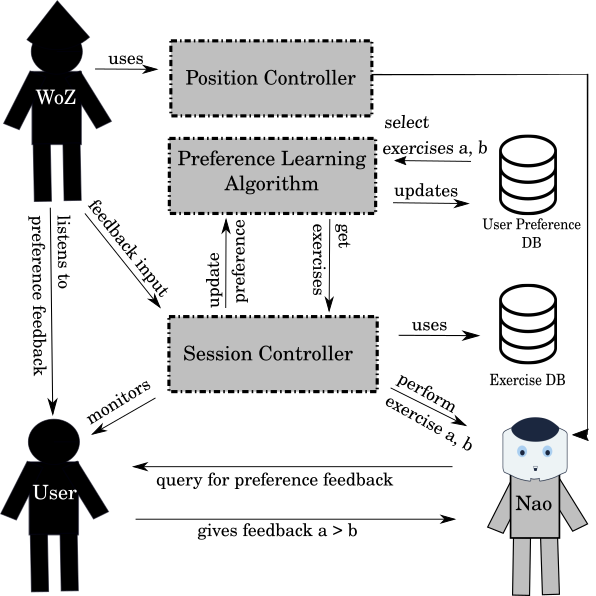
\includegraphics[width=\columnwidth]{figures/study.png}
\caption{System and interaction overview for the adaptive robot condition.} \label{fig:system}
\end{figure}


\subsection{Ecercise Database}
As previously found, exercising preference is individual for each person \cite{rhodes2006personality}. Thus, for the aim of this study, we developed a system that provides a variety of different exercises. We have chosen 25 exercises in total from 5 different categories: strength, stretch, cardio, Taichi, and meditation. This set of exercises tackles one of the open issues in SARs for exercising tasks.
Previous work often looked at a single type of exercise like arm movements \cite{eriksson2005hands,fasola2013socially,guneysu2017}. The approach of using a spectrum of different exercises might show that people can perform various exercises together with a robot.


\autoref{tab:pl:exercises} presents the list of the chosen exercises. They have been selected based on a variety of criteria: a) the possibility to animate and execute them on Nao (\ie{}, Nao cannot jump.), b) the difficulty that users can perform them (\ie{}, exercises should not be too challenging for the participants), c) the exercises should challenge the full embodiment of the robot (\ie{}, laying down, balancing, standing).

 All of them have been animated on Nao using Choregraphe \cite{gouaillier2008nao,pot2009choregraphe}. \autoref{fig:exercises} shows an example of a user exercising together with the robot.
 
 
\begin{table*}[t!]
\begin{center}

\caption{Used exercises for the presented study.}\label{tab:pl:exercises}
\begin{tabular}{@{} *5l @{}}    \toprule
% \emph{name} & \emph{foo} &&&&  \\\midrule
Strength  & Stretch & Cardio & Meditation & Taiji Drills \\ \midrule
  Push up & Neck    & Jumping Jacks & The boat & Golden rooster \\
Squats & Triceps & Front Lunge & 9 breathes & Rainbow\\
 Crunches & Hip  & Side Lunge & relaxation & Punch\\
 Superman & Quadriceps & Boxing & Inner light & Parting kick\\
 Bridge & Side  & Mnt. Climbers & Piece sign & Lifting water\\\bottomrule
% \bottomrule
\end{tabular}
\end{center}
\end{table*}

\begin{figure}[h!]
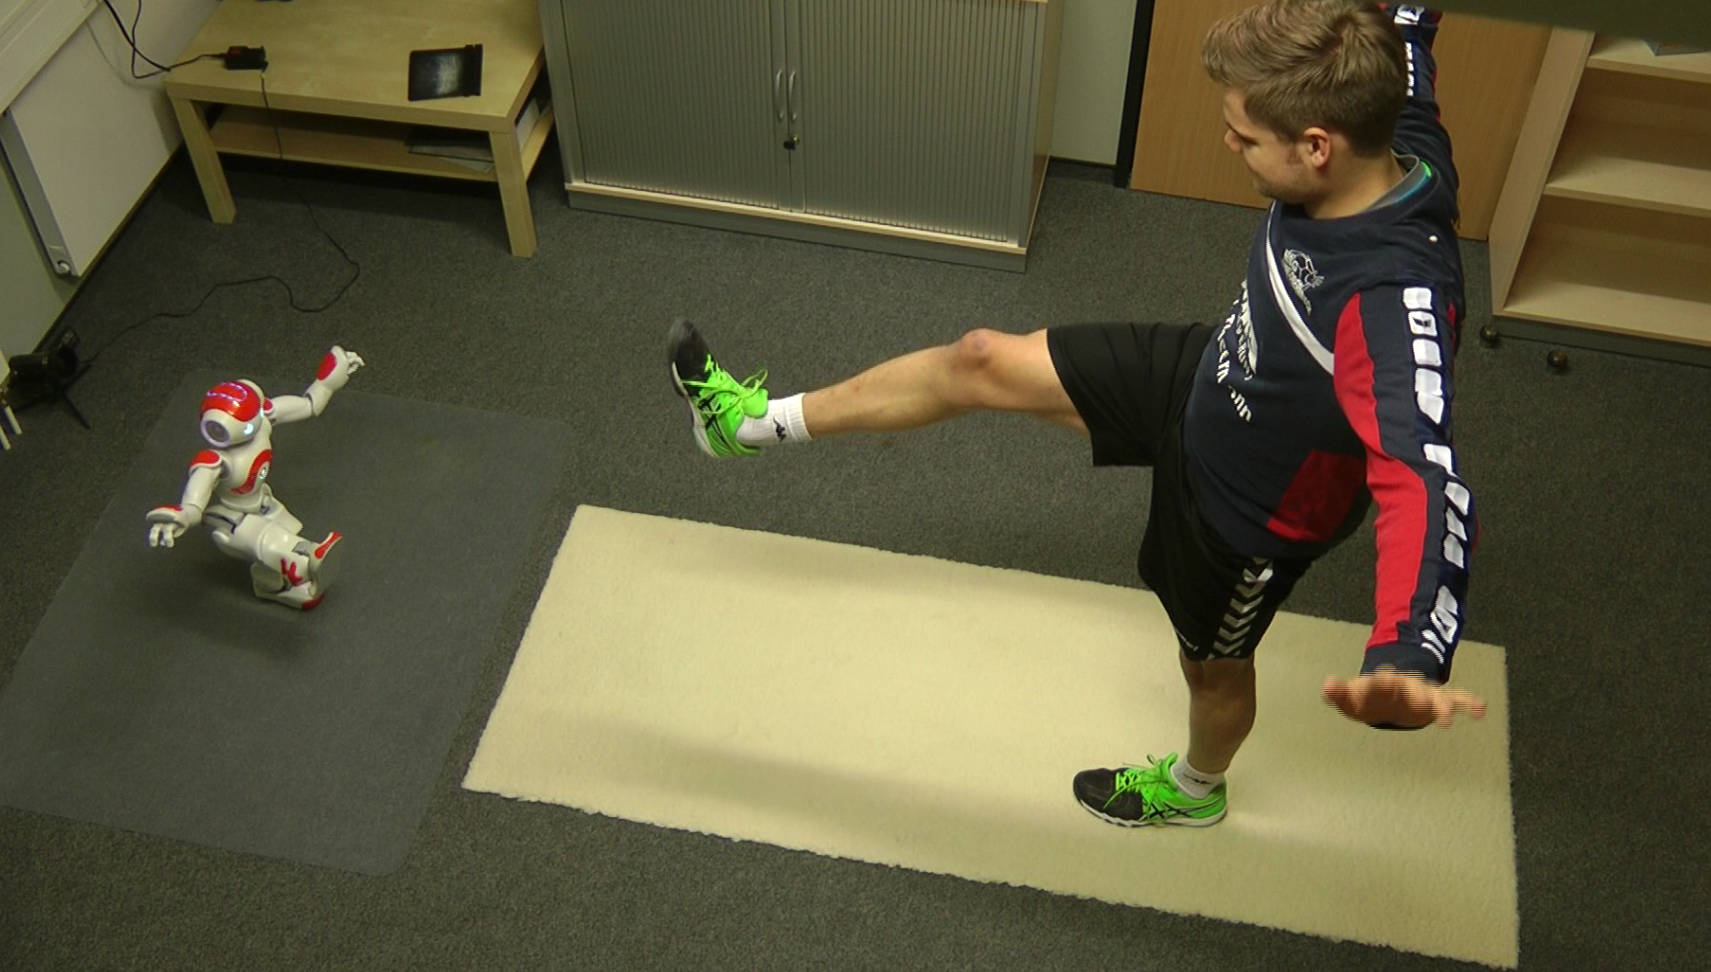
\includegraphics[width=\columnwidth]{figures/taichi.png}
\caption{Robot and user performing the Taiji drill \textit{Parting kick} together.} \label{fig:exercises}
\end{figure}


\subsection{Preference Learning Framework} \label{sec:framework}

This section will briefly introduce preference learning as a formal problem from the perspective of the Multi-Armed Bandit problem.

Preference learning is a subfield of machine learning that aims to learn predictive models from previously observed information (\ie{}, preference information) [@Fuernkranz2011]. 
In supervised learning, a data set of labeled items with preference information is used to predict preferences for new items or all the other items from a data set.
In general, the task for preference learning is concerned with the problem of learning to rank.


There are many different approaches to preference learning. 
It can be solved using supervised learning, unsupervised learning and also reinforcement learning. 
Since there exists no particular data set we could use for supervised or unsupervised learning, it is challenging to build a model that can predict preferences from previously observed information. 
Therefore, we are focusing on how the system can learn an initial preference relation for a given itemset without any prior information (\ie{}, the cold start problem). 
Thus, we are trying to solve the preference learning problem using online methods for the Multi-Armed Bandit problem or more precisely Dueling Bandit algorithms~\cite{yue2012k}.

The dueling bandit problem consists of $K$($K\geq2$) arms, where at each time step $t>0$ a pair of arms ($\alpha_{t}^{(1)},\alpha_{t}^{(2)}$) is drawn and presented to a user. A noisy comparison result $w_{t}$ is obtained, where $w_{t}=1$ if a user prefers $\alpha_{t}^{(1)}$ to $\alpha_{t}^{(2)}$, and $w_{t}=2$ otherwise. The distribution of the outcomes is presented by a preference matrix  $P=[p_{ij}]_{KxK}$, where $p_{ij}$ is the probability that a user prefers arm $i$ over arm $j$ (\eg{},$p_{ij} = P\{i\succ j\}, i,j = 1,2,..,K).$). 

The goal of the preference learning task is, given a set of different actions (\eg{}, different sport categories), to find the user's preference order for these categories by providing the user two $\alpha_{i}$ and $\alpha_{j}$ and update the user preferences based on the selection of the preference between $\alpha_i$ $\succ$ $\alpha_j$ or $\alpha_i$ $\prec$ $\alpha_j$.

Thus, the challenge is to find the user's preference by running an algorithm that balances the exploration (gaining new information) and the exploitation (utilizing the obtained information). In this work, we are using the Double Thompson Sampling (DTS) algorithm presented in~\cite{wu2016double}. 
Since there are several implementations to solve the dueling bandit problem we need to answer the question of why we have chosen this specific kind of algorithm.

Two reasons mainly drive this decision, the state of the art algorithms at the time of this study were DTS, RMED and its successor ECW-RMED~\cite{komiyama2015regret,komiyama2016copeland}. 
Both perform reasonably well regarding their asymptotic behavior. 
However, at this point, we are not interested in the long-term run of these algorithms but in the initial phase. 
If one takes a look at the first steps of these algorithms, one can see a significant difference between them that likely influence the HRI experience. 
RMED and ECW-RMED both have an initial phase where all possible pairs are repeatedly drawn for some time~\cite{komiyama2015regret,komiyama2016copeland} Algorithm 1. 
From an algorithmic perspective this is reasonable, but looking at it from the viewpoint of the interaction, this would lead to systematic comparisons that could result in boredom and even annoyance when the interaction partner is seemingly interrogating the user for her/his preferences. Thus, we assume that the DTS algorithm is more useful for HRI (especially for the initial contact between the trainee and the robot coach), because it does not rely on a systematic comparison of all possible pairs.


\subsection{Session Manager: System and Interaction Flow }
The session manager is also implemented using the presented framework from\cite{schneider2017framework}.

The system waits for a user to be present in the room. Depending on the distance, it asks the participant to come closer. The system intreoduces itself to the user, explains its behavior and asks whether the user wants to start the exercising program. Afterward, in the adaptive condition, the algorithm selects two exercises from the database, and Nao instructs the user to do the exercises. Following, it asks the participant which kind of exercises she or he prefers (preference feedback). 

At the beginning, we used the internal speech recognition of Nao. However, prototype experiments showed that the speech recognition capabilities are below an acceptable recognition rate, therefore we manually inserted the user's feedback using a Wizard of Oz (WoZ) style. 
Additionally, when Nao performs the exercises, it moves away from the initial position. We have implemented a simple marker based localization strategy. However, the robot needed too long to localize in the room and move to the correct position. Since it is a significant disturbance for the HRI experience, we also have implemented a WoZ position controller to move the robot to the correct position manually after each exercise. 

The primary interaction flow for the adaptive conditions is as follows: Based on the current user's preference database the algorithm selects two exercises, then the session manager runs these exercises sequentially. During the exercises, the session manager receives user skeleton information and monitors whether the user is doing the exercises. This exercising information was used to synchronize the exercising speed of the user and the robot. 
Afterward, the robot asks the user which of the exercises she or he prefers. The wizard listens to the user's feedback using an installed microphone in the experimental room and feeds the user's input back to the session manager. The robot acknowledges the decision by repeating the chosen exercise. The preference learning algorithm updates the user's preference database and selects the next exercises based on the current user preference. 

\section{Sudy Design} \label{adaptation:sec:study}

We conducted a study with a between-subject design (adaptive robot vs. adaptable robot) where participants were randomly assigned to one of two conditions. 

\subsection{Conditions}
\subsubsection{Adaptivity}
The robot in the adaptivity condition used the algorithm described in [@wu2016double]. During the introduction phase, the system explains to the user that it will do different exercises together with the user and will ask for preference feedback relating to the different exercises. At each time step, the system selects two exercises based and executed them consecutively with the user. Afterward, the system queries the user for a preference statement. This behavior repeated for 14 exercises (or seven iterations). After the 14 exercises, the system asks whether the user wants to continue exercising for two more exercises or quit the experiment. After the two additional exercises, the robot finishes the interaction. It states the user's learned preferences and thanks for the participation. We limited the additional exercises to two exercises, due to battery concerns and overheating of joints. 

\subsubsection{Adaptability}
The robot in the adaptability condition did not use any preference learning algorithm and did not select the next exercises autonomously. In the introduction phase, the system explains that it offers different exercises they can do together. The robot verbally listed the possible exercising categories in a randomized order and the user could choose the exercise category she or he wants to experience. Thus, the user was in control of the exercise session and could choose the exercise category she or he prefers. Also in this condition, the human and robot did 14 exercises together, and the robot asked whether the user wants to do two additional exercises. 

\subsection{Participants}
Participants ($N$ = 40; average age $M$ = 26.02, $SD$ = 5.48, 13 female and 7 male  in the adaptivity condition; 12 female and 8 male in the adaptability condition) were mostly university students that were acquired by information on the campus and social media. The majority of the participants were naive robot user and had no background in computer engineering or programming.

\subsection{Procedure}
Participants arrived at the lab individually. 
First, they had to sign a consent form. 
Then, the experimenter led the participants to a room where they can change their clothes. 
Later, they were told to enter the lab and follow the instructions of the system. Until this point, the participants did not know that they will be interacting with a robotic system. We neglected this prior information to not bias the participants or raise false beliefs. Then the participants entered the lab without the experimenter. The interaction happened for approximately 40 minutes, and the experimenter monitored the experiment from a control room. After the interaction finished, participants had to answer a questionnaire and had a short interview. Finally, they were debriefed and received 8 Euros for their participation. The ethical committee of our university approved the procedure.

\begin{acknowledgements}
If you'd like to thank anyone, place your comments here
and remove the percent signs.
\end{acknowledgements}

\printbibliography{}

% BibTeX users please use one of
%\bibliographystyle{spbasic}      % basic style, author-year citations
%\bibliographystyle{spmpsci}      % mathematics and physical sciences
% \bibliographystyle{spphys}       % APS-like style for physics
% \bibliography{mybibfile}   % name your BibTeX data base

% Non-BibTeX users please use
% \begin{thebibliography}{}
% %
% % and use \bibitem to create references. Consult the Instructions
% % for authors for reference list style.
% %
% \bibitem{RefJ}
% % Format for Journal Reference
% Author, Article title, Journal, Volume, page numbers (year)
% % Format for books
% \bibitem{RefB}
% Author, Book title, page numbers. Publisher, place (year)
% % etc
% \end{thebibliography}

\end{document}
% end of file template.tex

